After the experiment with only one lighting dot, the next step is using several lighting points. Thus, the goal of this experiment is using multiple points in order to detect several distances in front of the camera.

\subsection{Choices of Implementation}
First of all, a grid of dots is supposed to be projected on the target. However, instead of a grid, a line of 10 dots is used during this experiment. Indeed, as the triangulation theory between a grid and a line of dots is the same and the indexing of the dots of a grid is much more difficult than the one of the dots of a line, it has been chosen to use a line in order to focus on the improvement of the robustness and accuracy of the algorithm. 

Then, as the purpose of this project is the vision analysis, the focus is on the structured light algorithm and the artificial light source has not been built. Thus, in order to be able to project a line of several dots on a target, it has been chosen to use a overhead projector. Indeed, even if a laser was available (see the first experiment), after trying to diffract its beam (using a CD for instance), it appeared that the brightness of each dot was very imbalanced (central dot very luminous compared to the others) and would lead to a modification of the parameters of the dot detection. Moreover, as the artificial light source is supposed to project a grid of identical dots, the overhead projector has been chosen to respect this equality of brightness.


\subsection{Progress of the Experiment}
A picture of a line of 10 green dots (a green close to the one of the laser) with a reddish background (in order to represent the color of the rocks of Mars) is projected on a board using the overhead projector. Then an object is placed between the board and the camera and the several distances $z_i$ are computed (see Figure \ref{fig:expGridSchema}).


\begin{figure}[H]
  %\centering
  \centerline{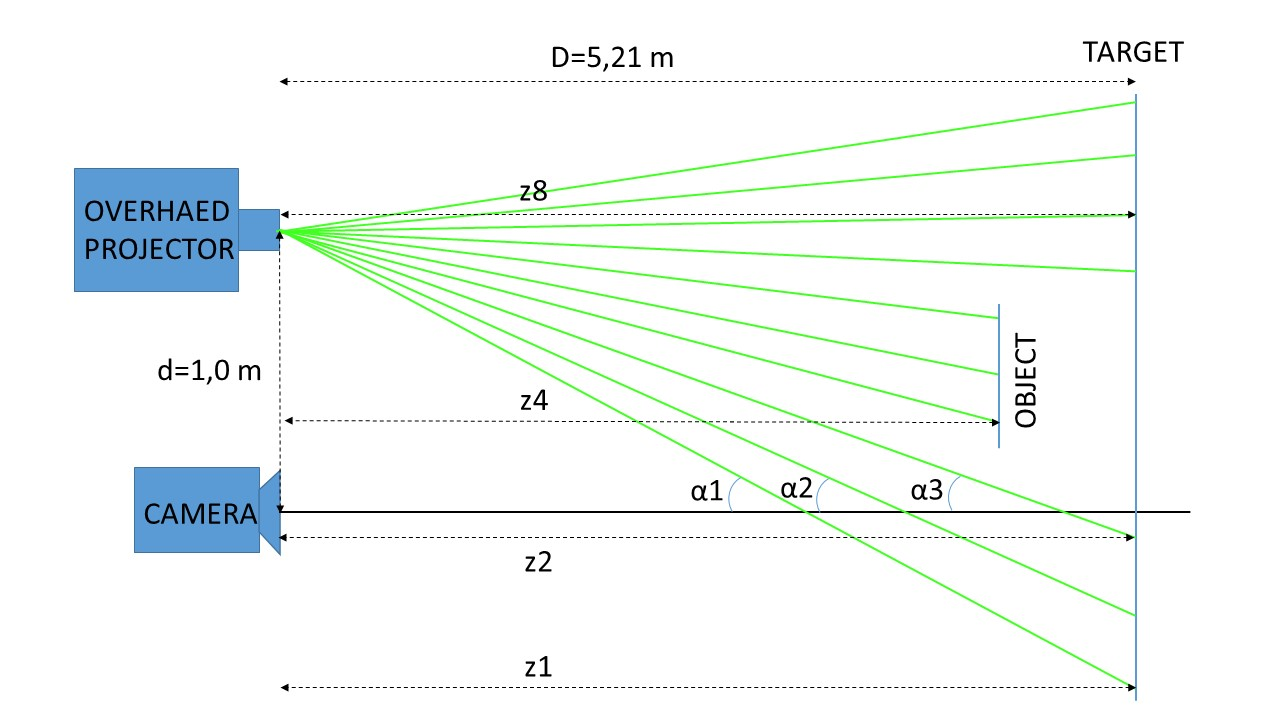
\includegraphics[scale=0.4]{fig/expGridSchema.jpg}}
  \caption{schema of the experiment}
  \label{fig:expGridSchema}
\end{figure}


Once the script is run, the different steps are the following :
\paragraph*{Step 1 : Calibration}
~~\\
In order to find the different angles $\alpha_i$ between the focal axis of the camera and the beams of the projector, a calibration function is called before the real time loop. This function detects the lighting dots, their centroid and use the following formula to save the different $\tan \alpha_i$ into an array:

\begin{equation*}
\tan \alpha_i = \frac{d}{D}-P_{pixels,i}\frac{P_{size}}{f_0}
\end{equation*}


\paragraph*{Step 2 : Positioning of the Object}
~~\\
During this step, while the script is still running, the object is placed between the camera and the board (see Figure \ref{fig:positioningObject}). On the one hand, as the projector is higher than the camera, it makes the $9^{th}$ dot slides vertically. However, it does not affect the result as only the horizontal slide is taken into account and the \emph{sort} function permits to keep the dots in the right order even if they slide vertically. On the other hand, a horizontal slide occurs as expected.

The experiment has been carried out with several distances and placement of the object in front of various dots. Moreover, some noise has been added. As we can see figure \ref{fig:positioning70Object}, the background is nuanced, smaller dots with the same green are added and dots of the same size but with others greens are added too. We can see figure \ref{fig:expGrid70HSV} that the algorithm manages to filter the different noises and still detects the 10 dots.



\begin{figure}[!h] 
\centering
\subfigure[Positioning of the object in front of the $9^{th}$ dot]{
  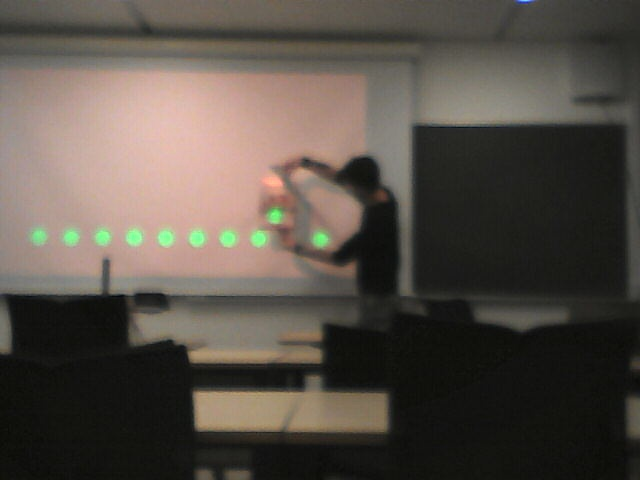
\includegraphics[scale=0.30]{fig/positioning50Object.jpg}
  \label{fig:positioningObject}
}
\quad 
\subfigure[Detection of the centroids]{
  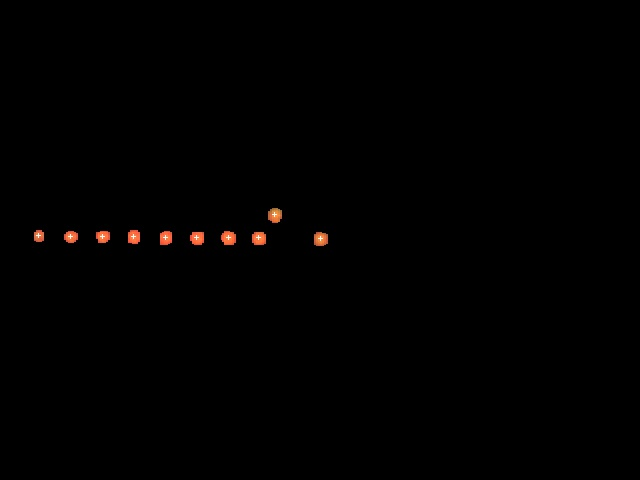
\includegraphics[scale=0.30]{fig/expGrid50HSV.jpg}
  \label{fig:expGridHSV}
}
\caption{Distance object-board = 50 cm}
\end{figure}

\begin{figure}[!h] 
\centering
\subfigure[Positioning of the object in front of the $6^{th}$ and $7^{th}$ dots]{
  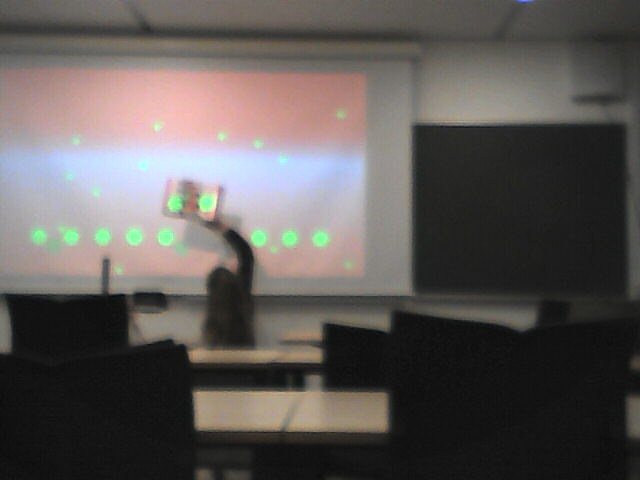
\includegraphics[scale=0.30]{fig/grid70.jpg}
  \label{fig:positioning70Object}
}
\quad 
\subfigure[Detection of the centroids]{
  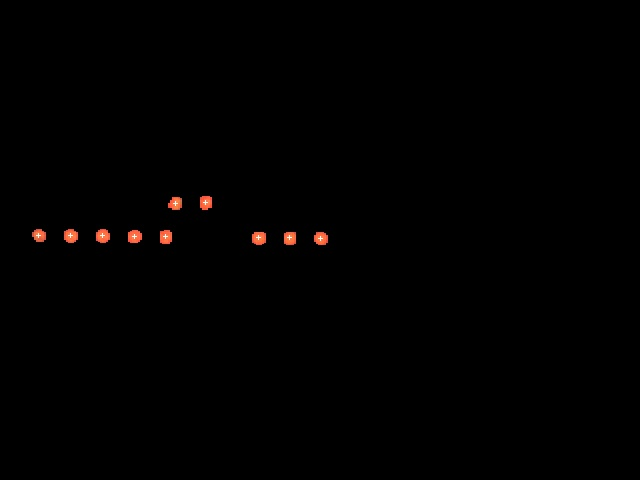
\includegraphics[scale=0.30]{fig/grid70HSV.jpg}
  \label{fig:expGrid70HSV}
}
\caption{Distance object-board = 90 cm}
\end{figure}


This experiment was carried out in real time, that is to say the several distances were displayed continuously. However, some pictures were saved in order to permit people to run the algorithm used during the experiment. Indeed, you can find into the folder '???????' the C++ script used and pictures of objects at several distances taken by the camera. Moreover, the Power Point employed to project the dots and backgrounds are also present in order to permit the performing of the experiment in real time but in this case, the distances camera-projector \emph{d} and camera-target \emph{D} need to be adapted and the calibration done.


\subsection{Results}
The results of the experiment for the different distances object-board are presented Tables \ref{res50cm}, \ref{res50cm2}, \ref{res90cm} and \ref{res70cm}.

\begin{table}[H]
\centering
\caption{Object in front of dot 9 with distance object-board = 0.50 m (without noise)}
\label{res50cm}
\renewcommand{\arraystretch}{1.5}
\begin{tabular}{|c|c|c|c|c|c|}
\hline
i & $z_i$ [m] & error\footnotemark[1] [\%] & distance board-Object [m] & error\footnotemark[1] [\%] \\
\hline
1 & 5.16205 & 0.92 & 0.048 & \\
\hline
2 & 5.18899 & 0.40 & 0.021 & \\
\hline
3 & 5.20282 & 0.14 & 0.007 & \\
\hline
4 & 5.20879 & 0.02 & 0.001 & \\
\hline
5 & 5.20999 & 0.00 & 0.000 & \\
\hline
6 & 5.17524 & 0.67 & 0.035 & \\
\hline 
7 & 5.21324 & 0.06 & -0.003 & \\
\hline
8 & 5.22243 & 0.24 & -0.012 & \\
\hline
9 & 4.75529 & 0.01 & 0.455 & 9.06 \\
\hline
10 & 5.27336 & 1.22 & -0.063 & \\
\hline
\end{tabular}
\end{table}
\footnotetext[1]{$error = \frac{distance_{theory}-distance_{experiment}}{distance_{theory}}100$}

\begin{table}[H]
\centering
\caption{Object in front of dots 1 and 2 with distance object-board = 0.50 m (without noise)}
\label{res50cm2}
\renewcommand{\arraystretch}{1.5}
\begin{tabular}{|c|c|c|c|c|c|}
\hline
i & $z_i$ [m] & error [\%] & distance board-Object [m] & error [\%] \\
\hline
1 & 4.69081 & 0.41 & 0.519 & 3.84 \\
\hline
2 & 4.74072 & 0.65 & 0.469 & 6.14 \\
\hline
3 & 5.20312 & 0.13 & 0.007 & \\
\hline
4 & 5.17385 & 0.69 & 0.036 & \\
\hline
5 & 5.20999 & 0.00 & 0.000 & \\
\hline
6 & 5.2103 & 0.01 & -0.000 & \\
\hline 
7 & 5.21342 & 0.07 & -0.003 & \\
\hline
8 & 5.22243 & 0.24 & -0.012 & \\
\hline
9 & 5.24131 & 0.60 & -0.031 & \\
\hline
10 & 5.30847 & 1.89 & -0.098 & \\
\hline
\end{tabular}
\end{table}



\begin{table}[H]
\centering
\caption{Object in front of dots 1 and 2 with distance object-board = 0.90 m (without noise)}
\label{res90cm}
\renewcommand{\arraystretch}{1.5}
\begin{tabular}{|c|c|c|c|c|c|}
\hline
i & $z_i$ [m] & error [\%] & distance board-Object [m] & error [\%] \\
\hline
1 & 4.34553 & 0.82 & 0.864 & 3.95 \\
\hline
2 & 4.36417  & 1.26 & 0.846 & 6.02 \\
\hline
3 & 5.23825 & 0.54 & -0.028 & \\
\hline
4 & 5.2443 & 0.66 & -0.034 & \\
\hline
5 & 5.20999 &	0.00 & 0.000 & \\
\hline
6 & 5.17524 &	0,67 & 0,035 & \\
\hline
7 & 5.21324	& 0,06 & -0,003 & \\
\hline
8 & 5.22243	& 0,24 & -0,012 & \\
\hline
9 & 5.27727	& 1,29 & -0,067 & \\
\hline
10 & 5.23746 & 0,53 &	-0,027 & \\
\hline
\end{tabular}
\end{table}


\begin{table}[H]
\centering
\caption{Object in front of dots 6 and 7 with distance object-board = 0.70 m and noise}
\label{res70cm}
\renewcommand{\arraystretch}{1.5}
\begin{tabular}{|c|c|c|c|c|c|}
\hline
i & $z_i$ [m] & error [\%] & distance board-Object [m] & error [\%] \\
\hline
1 & 5.16204 & 0.92 & 0.048 & \\
\hline
2 & 5.18898 & 0.40 & 0.021 & \\
\hline
3 & 5.20312 & 0.13 & 0.007 & \\
\hline
4 & 5.20879 & 0.02 & 0.001 & \\
\hline
5 & 5.20999 & 0.00 & 0.000 & \\
\hline
6 & 4.53458 & 0.55 & 0.675 & 3.51 \\
\hline
7 & 4.51034 & 0.01 & 0.700 & 0.04 \\
\hline
8 & 5.22242 & 0.24 & -0.012 & \\
\hline
9 & 5.24131 & 0.60 & -0.031 & \\
\hline
10 & 5.30848 & 1.89 & -0.09848 & \\
\hline
\end{tabular}
\end{table}


\subsection{Interpretations}
As we can see on the Table \ref{res70cm}, the errors of the results of the experiment with noise are in the same order of magnitude than the ones without noise. It means that the algorithm is robust enough to handle the noise. Indeed, the 
opening permitting the selection of only the dots of the projected pattern works well. Moreover, as we can see figure \ref{fig:positioningObject} and \ref{fig:positioning70Object}, the images recorded are very blurred because of the camera used (webcam Philips SPZ2000). As the results are acceptable, it means that the algorithm deals also with the blur, that is to say that it could even work if the target gets a bit out of the depth of field.

However, according to the four Tables, we can see that the errors of the distance object-board is between 0.04 and 9.06 \%, which can be a significant error. Indeed, an error of 9.06 \% represents an experimental distance of 455 mm instead of 500 which means an error of 45 mm. For instance, our target is supposed to be a rock at a distance between one and two meters. Let us assume that one of the projected dots is on a part of the rock which is 1500 mm far from the camera. An error of 9.06 \% would lead to a measured distance of 1364 mm, that is to say an error of 136 mm. To have a negligible error, the rock should have a shape such as the depth would vary over a range of at least one meter. Therefore, it would definitely not be acceptable.

These errors come from the calibration and the detection of the centroids. Regarding the calibration, we have to notice that during this experiment, it was not rigorous. Indeed, the distances board-object, \emph{D} and \emph{d} were measured with a measure tape which is not precise enough. Also, the focal axis of the camera was not exactly perpendicular to the target as it is supposed to be according to the delimitation of the scene. Therefore, the errors of the measurements of the distances should decrease with a precise calibration done with adapted tools. As the overhead projector was fixed on the ceiling and the focal axis of the camera had to stay perpendicular to the target, we were not able to make the distance \emph{d} vary. It could have been interesting to make the angles $\alpha$ vary in order to study the precision of the results according to these angles. Indeed, a bigger angle $\alpha$ would lead to a bigger distance \emph{p} and thus variations of the centroids would have been more negligible.

Moreover, several aspects of the detection of the centroids could be improved. The main one is that, as the brightness of the lighting dots is not uniform, that is to say it decreases with the distance from the center, the algorithm of color detection does not detect the same pixels over time, some bordering pixels are detected or not over time. This weakness of the color detection changes the position of the centroids and leads to a bigger error. Indeed, the experiment from Table \ref{res50cm} has been done again (using the capture of the image recorded by the camera during the experiment in order to compute exactly the same distances and get the same results) but subtracting one pixel to the distance \emph{p} between the image of the object on the CCD sensor and the geometrical center of the CCD. This subtraction simulates an error of one pixel to the left of the position of centroid computed. The result of this experiment is that the new distance board-object is now 0.484 m instead of 0.455 m and the error decreases significantly from 9.06\% to 3.22\%. In this case, one pixel represents an error of 29 mm, that is to say an error of almost 6\%. The same experiment has been done with the image of the experiment from Table \ref{res70cm} and the errors change from 3.51\% to 0.28\% and 0.04\% to 3.71\%. One pixel represents an error of approximately 3.77\%. Finally, using the experiment Table \ref{res90cm}, one pixel represents an error of almost 2.69\%. The error caused by one pixel on the distance target-board has been calculated for 3 different values of $\tan \alpha$ (see Figure \ref{fig:error}). As we can see, when $\tan \alpha$ is equal to 0.1919, the errors match with the values obtained during the experiment. Moreover, this graphic shows that even if $\tan \alpha$ does not matter for big distances board-target with the target close to the camera, the error caused by one pixel is very important when the target is near the calibration distance, that is to say 5.21m. It makes sense because at such a distance, \emph{p} is supposed to be zero so the error will be much more accentuated. We can conclude that, as the target is a rock with a relief inferior than 50 cm, the system needs to be accurate for short relief and the error will be minimized using a distance \emph{d} camera-Artificial Light Source as big as possible.


\begin{figure}[H]
  %\centering
  \centerline{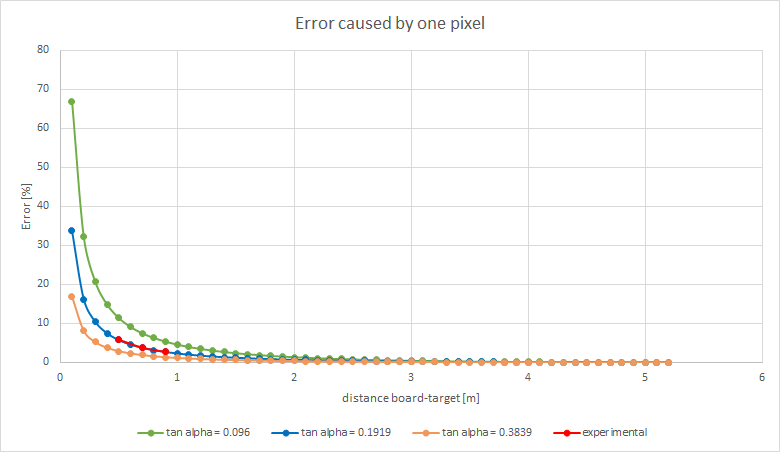
\includegraphics[scale=0.7]{fig/error.png}}
  \caption{error on the distance board-target caused by one pixel}
  \label{fig:error}
\end{figure}



\subsection{Limits of the Experiment}
The first limit of this experiment is that some pattern disorders are not taken into account. The permutation of dots that can happen with an object too far from the board has been prevented with a maximum distance board-object = 90 cm. With a greater distance than one meter, a permutation appears between the dots on the object and the ones at the left of the object but this permutation is not managed, not corrected by the \emph{sort} function. Another disorder not tested is the merge of two dots. As the projector was on the ceiling, projecting slightly downward, the dots shifted horizontally but also vertically and as a consequence, the dots on the object were to high to merge with the dots on the board. Even if this kind of disorder was tested during the integration tests \ref{centroiding}, it would have been interesting to test it during the experiment.
A second limit is that, as this experiment does not include several aspects of the system designed (projector instead of the artificial light source, line of dots instead of a grid, ...), it cannot be considered as a test of this last one. Nevertheless, it permits to test the accuracy and the robustness of the algorithm tested. It is only an integration test.





